% Options for packages loaded elsewhere
\PassOptionsToPackage{unicode}{hyperref}
\PassOptionsToPackage{hyphens}{url}
\PassOptionsToPackage{dvipsnames,svgnames,x11names}{xcolor}
%
\documentclass[
  letterpaper,
  DIV=11,
  numbers=noendperiod]{scrartcl}

\usepackage{amsmath,amssymb}
\usepackage{iftex}
\ifPDFTeX
  \usepackage[T1]{fontenc}
  \usepackage[utf8]{inputenc}
  \usepackage{textcomp} % provide euro and other symbols
\else % if luatex or xetex
  \usepackage{unicode-math}
  \defaultfontfeatures{Scale=MatchLowercase}
  \defaultfontfeatures[\rmfamily]{Ligatures=TeX,Scale=1}
\fi
\usepackage{lmodern}
\ifPDFTeX\else  
    % xetex/luatex font selection
\fi
% Use upquote if available, for straight quotes in verbatim environments
\IfFileExists{upquote.sty}{\usepackage{upquote}}{}
\IfFileExists{microtype.sty}{% use microtype if available
  \usepackage[]{microtype}
  \UseMicrotypeSet[protrusion]{basicmath} % disable protrusion for tt fonts
}{}
\makeatletter
\@ifundefined{KOMAClassName}{% if non-KOMA class
  \IfFileExists{parskip.sty}{%
    \usepackage{parskip}
  }{% else
    \setlength{\parindent}{0pt}
    \setlength{\parskip}{6pt plus 2pt minus 1pt}}
}{% if KOMA class
  \KOMAoptions{parskip=half}}
\makeatother
\usepackage{xcolor}
\setlength{\emergencystretch}{3em} % prevent overfull lines
\setcounter{secnumdepth}{-\maxdimen} % remove section numbering
% Make \paragraph and \subparagraph free-standing
\ifx\paragraph\undefined\else
  \let\oldparagraph\paragraph
  \renewcommand{\paragraph}[1]{\oldparagraph{#1}\mbox{}}
\fi
\ifx\subparagraph\undefined\else
  \let\oldsubparagraph\subparagraph
  \renewcommand{\subparagraph}[1]{\oldsubparagraph{#1}\mbox{}}
\fi


\providecommand{\tightlist}{%
  \setlength{\itemsep}{0pt}\setlength{\parskip}{0pt}}\usepackage{longtable,booktabs,array}
\usepackage{calc} % for calculating minipage widths
% Correct order of tables after \paragraph or \subparagraph
\usepackage{etoolbox}
\makeatletter
\patchcmd\longtable{\par}{\if@noskipsec\mbox{}\fi\par}{}{}
\makeatother
% Allow footnotes in longtable head/foot
\IfFileExists{footnotehyper.sty}{\usepackage{footnotehyper}}{\usepackage{footnote}}
\makesavenoteenv{longtable}
\usepackage{graphicx}
\makeatletter
\def\maxwidth{\ifdim\Gin@nat@width>\linewidth\linewidth\else\Gin@nat@width\fi}
\def\maxheight{\ifdim\Gin@nat@height>\textheight\textheight\else\Gin@nat@height\fi}
\makeatother
% Scale images if necessary, so that they will not overflow the page
% margins by default, and it is still possible to overwrite the defaults
% using explicit options in \includegraphics[width, height, ...]{}
\setkeys{Gin}{width=\maxwidth,height=\maxheight,keepaspectratio}
% Set default figure placement to htbp
\makeatletter
\def\fps@figure{htbp}
\makeatother

\KOMAoption{captions}{tableheading}
\makeatletter
\makeatother
\makeatletter
\makeatother
\makeatletter
\@ifpackageloaded{caption}{}{\usepackage{caption}}
\AtBeginDocument{%
\ifdefined\contentsname
  \renewcommand*\contentsname{Table of contents}
\else
  \newcommand\contentsname{Table of contents}
\fi
\ifdefined\listfigurename
  \renewcommand*\listfigurename{List of Figures}
\else
  \newcommand\listfigurename{List of Figures}
\fi
\ifdefined\listtablename
  \renewcommand*\listtablename{List of Tables}
\else
  \newcommand\listtablename{List of Tables}
\fi
\ifdefined\figurename
  \renewcommand*\figurename{Figure}
\else
  \newcommand\figurename{Figure}
\fi
\ifdefined\tablename
  \renewcommand*\tablename{Table}
\else
  \newcommand\tablename{Table}
\fi
}
\@ifpackageloaded{float}{}{\usepackage{float}}
\floatstyle{ruled}
\@ifundefined{c@chapter}{\newfloat{codelisting}{h}{lop}}{\newfloat{codelisting}{h}{lop}[chapter]}
\floatname{codelisting}{Listing}
\newcommand*\listoflistings{\listof{codelisting}{List of Listings}}
\makeatother
\makeatletter
\@ifpackageloaded{caption}{}{\usepackage{caption}}
\@ifpackageloaded{subcaption}{}{\usepackage{subcaption}}
\makeatother
\makeatletter
\@ifpackageloaded{tcolorbox}{}{\usepackage[skins,breakable]{tcolorbox}}
\makeatother
\makeatletter
\@ifundefined{shadecolor}{\definecolor{shadecolor}{rgb}{.97, .97, .97}}
\makeatother
\makeatletter
\makeatother
\makeatletter
\makeatother
\ifLuaTeX
  \usepackage{selnolig}  % disable illegal ligatures
\fi
\IfFileExists{bookmark.sty}{\usepackage{bookmark}}{\usepackage{hyperref}}
\IfFileExists{xurl.sty}{\usepackage{xurl}}{} % add URL line breaks if available
\urlstyle{same} % disable monospaced font for URLs
\hypersetup{
  colorlinks=true,
  linkcolor={blue},
  filecolor={Maroon},
  citecolor={Blue},
  urlcolor={Blue},
  pdfcreator={LaTeX via pandoc}}

\author{}
\date{}

\begin{document}
\ifdefined\Shaded\renewenvironment{Shaded}{\begin{tcolorbox}[enhanced, frame hidden, boxrule=0pt, sharp corners, interior hidden, breakable, borderline west={3pt}{0pt}{shadecolor}]}{\end{tcolorbox}}\fi

\hypertarget{a-stylometric-analysis-of-the-book-of-mormon}{%
\section{A Stylometric Analysis of The Book of
Mormon}\label{a-stylometric-analysis-of-the-book-of-mormon}}

\textbf{By: Joseph Allen}

\begin{center}\rule{0.5\linewidth}{0.5pt}\end{center}

\hypertarget{description}{%
\section{Description}\label{description}}

Stylometry is the statistical analysis of variations in literary style
between writers. One of the most controversial texts of the 1800's is
Joseph Smith's ``The Book of Mormon' Joseph Smith's claim regarding the
text is that he translated it from an ancient record. He also claims
that translation process was done through miraculous means. Looking at
The Book of Mormon we see that the text claims multiple unique
authorship. Critics would claim a naturalistic approach for The Book of
Mormon meaning that Joseph Smith did not have any miraculous means to
write The Book of Mormon and instead wrote it through his own abilities
and intellect.

\hypertarget{purpose}{%
\section{Purpose}\label{purpose}}

The goal is to use stylometric methods to analyze The Book of Mormon and
explore its claims of diverse authorship. Additionally, we aim to
compare it to other contemporary texts, including those written by
Joseph Smith and his contemporaries, using modern data analysis
techniques.

\hypertarget{scope-and-overview}{%
\section{Scope and Overview}\label{scope-and-overview}}

This analysis will cover: - The Book of Mormon - Other writings by
Joseph Smith (e.g., Doctrine and Covenants, Pearl of Great Price) -
Texts from the same era that critics often claim would be possible
sources Joseph Smith used to write The Book of Mormon (The Late War,
Spaulding Manuscripts, View of The Hebrews) - New Testament

Using machine learning and data visualization, we will: - Compare
authorship within The Book of Mormon - Compare The Book of Mormon to
Joseph Smith's other writings - Compare The Book of Mormon to other
19th-century texts - Compare The Book of Mormon to the New Testament -
Compare all the text to each other.

We will focus on stylometric variables such as: - Function words -
Average letters used per word - Average words used per sentence -
Individual letter usage

The usage of function words provide us some very useful info in
determining of authorship. In an article written by Mike Kestemont,
``Function Words in Authorship Attribution From Black Magic to Theory?''
He provides some useful points as to why function words are useful for
this analysis.

\begin{itemize}
\item
  ``All authors writing in the same language and period are bound to use
  the very same function words. Function words are therefore a reliable
  base for textual comparison;''
\item
  ``Their high frequency makes them interesting from a quantitative
  point of view, since we have many observations for them;''
\item
  ``The use of function words is not strongly affected by a text's topic
  or genre: the use of the article `the', for instance, is unlikely to
  be influenced by a text's topic.''
\item
  ``The use of function words seems less under an author's conscious
  control during the writing process.''
\item
  ``Recall the last advantage listed above: the argument is often raised
  that the use of these words would not be under an author's conscious
  control during the writing process (Stamatatos, 2009; Binongo, 2003;
  Argamon and Levitan, 2005; Peng et al., 2003). This would indeed help
  to explain why function words might act as an author invariant
  throughout an oeuvre (Koppel et al., 2009, p.~11). Moreover, from a
  methodological point of view, this would have to be true for forgers
  and imitators as well, hence, rendering function words resistant to
  stylistic imitation and forgery.''
\end{itemize}

Mike Kestemont writes about this idea that function words are used by
and author subconsciously, and an author's usage of them can help reveal
imitations and forgeries.

\hypertarget{methodology}{%
\section{Methodology}\label{methodology}}

\begin{enumerate}
\def\labelenumi{\arabic{enumi}.}
\tightlist
\item
  \textbf{Problem Definition}: Stylometric analysis of The Book of
  Mormon and other contemporary text.
\item
  \textbf{Data Collection}: Gather texts from The Book of Mormon and
  other relevant sources.
\item
  \textbf{Data Exploration and Preprocessing}: Prepare the text for
  analysis.
\item
  \textbf{Data Analysis}: Visualize various stylometric variables.
\item
  \textbf{Modeling}: Train machine learning models to test authorship.
\item
  \textbf{Model Evaluation}: Validate model performance.
\item
  \textbf{Results Communication}: Present findings.
\end{enumerate}

\hypertarget{data-preprocessing-process}{%
\section{Data Preprocessing Process}\label{data-preprocessing-process}}

My goal was to extract stylometric variables out of the text according
to authorship. This involved first involved gathering all writings and
annotating them to their associated authors. From there I was able to
divide the writings into subsets based on how much training data I
wanted.

For each author grouping of verses, I extracted the following
stylometric variables out of the text:

\begin{itemize}
\tightlist
\item
  Individual function word use frequency compared to all words
\item
  Individual function word use frequency compared to all function
  words.'
\item
  Overall function word use percentage
\item
  Total word count
\item
  Total function word count
\item
  Letter use percentages
\item
  Average letters per word
\item
  Average word per verse
\end{itemize}

I was able to get all this information to be dynamically created and
generated into CSV files.

\hypertarget{authorship-note}{%
\subsection{Authorship note}\label{authorship-note}}

For all datasets except The Pearl of Great Price I just went with the
traditional authorship. For The Pearl of Great Price since there is some
difference in how a text was authored, such as claims of translation to
just a dictation of Joseph Smith's words I just had authorship tied to
the book it came frame, except for Joseph Smith History and The Articles
of Faith which are tied to the authorship ``Joseph Smith''

\hypertarget{modeling}{%
\section{Modeling}\label{modeling}}

I used four different machine learning models in my analysis. All those
models predict categorically meaning that they would guess an author
given some data. The models I used are the following: - Random Forst - K
Nearest Neighbors - Neural Network - Ensemble Model

It is also important to note that the Ensemble Model is basically just a
combination of the other three models.

Explaining how each model works is out of the scope of the process, but
it is sufficient to say that each model uses different statistical
methods to define patterns that it finds in data, and then makes
predictions based off those patterns.

The metrics we use to evaluate the model's performance are accuracy,
precision, recall, and f1 score. They are defined as:

\begin{itemize}
\tightlist
\item
  Accuracy: The proportion of all predictions (both positive and
  negative) that were correct.
\item
  Precision: The proportion of predicted positives that were correct.
\item
  Recall: The proportion of actual positives that were correctly
  identified.
\item
  F1 Score: The harmonic mean of precision and recall, balancing the
  two. (Per OpenAI. (2024). ChatGPT conversational AI model.)
\end{itemize}

While all of these metrics are useful, the most useful metrics for us to
look at is accuracy and f1 score.

\hypertarget{modeling-methods}{%
\subsection{Modeling Methods}\label{modeling-methods}}

I created nine different subsets of data containing the following
datasets: - All available datasets - All available datasets except the
New Testament - The Book of Mormon by itself - The Book of Mormon and
Doctrine \& Covenants - The Book of Mormon and New Testament - The Book
of Mormon, The Late War, Spaulding Manuscript, and The View of The
Hebrews - The Book of Mormon and Pearl of Great Price - The Doctrine \&
Covenants, The Late War, Spaulding Manuscript, and The View of The
Hebrews - The New Testament by itself.

\hypertarget{findings}{%
\section{Findings}\label{findings}}

\hypertarget{model-performance}{%
\subsection{\texorpdfstring{\textbf{Model
Performance}}{Model Performance}}\label{model-performance}}

In terms of performance the models consistently ranked in the order of

\begin{enumerate}
\def\labelenumi{\arabic{enumi}.}
\tightlist
\item
  Random Forest
\item
  K Nearest Neighbors
\item
  Ensemble Model
\item
  Neural Network
\end{enumerate}

The models perform quite well when it comes to authors/text that had a
higher amount of data. Inversely, the models perform much worse on
authors/text that had lower amounts of data. This would be authors such
as Enos, Joseph Smith History, Joseph Smith's Revision of Matthew,
Articles of Faith, The Book of Moses, James and Peter. Notably, The
Pearl of Great Price text was wildly inconsistent, almost getting scores
of near 0\% accuracy for some authors.

We can view the performance of the models in two ways: through the raw
metrics numbers and through a confusion matrix. A confusion matrix shows
how each author performed in the model. This is valuable information as
it allows us to see how the model is specifically working/messing up.
Since the Random Forest model performed the best, we will look at the
performance of that model against the different datasets. For
interpretation of a confusion matrix a simple way to look at it is the
higher the numbers on the diagonal the better.

\hypertarget{the-book-of-mormon-authorship}{%
\subsubsection{\texorpdfstring{\emph{The Book of Mormon
Authorship}}{The Book of Mormon Authorship}}\label{the-book-of-mormon-authorship}}

\begin{figure}

{\centering 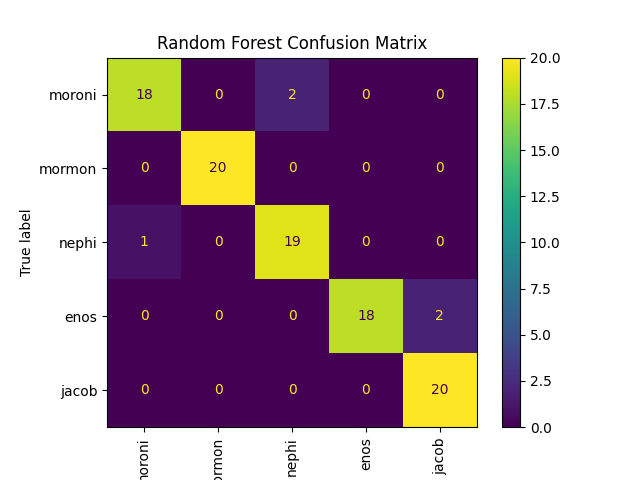
\includegraphics{Graphs/BoM/rf.png}

}

\caption{BoM Random Forest Confusion Matrix}

\end{figure}

\begin{itemize}
\tightlist
\item
  Accuracy: 0.9400
\item
  Precision: 0.9434
\item
  Recall: 0.9400
\item
  F1-Score: 0.9398
\end{itemize}

As you can see with just predicting within The Book of Mormon the Random
Forest model does extremely well at predicting authorship! This supports
the idea that the different claimed authors of The Book of Mormon have
unique enough writing styles from each other that they can be accurately
predicted by a Random Forest Model.

We can see that when including Joseph Smith's writings as found in
Doctrine and Covenants, this pattern continues.

\begin{figure}

{\centering \includegraphics{Graphs/BoM\&D\&C/rf.png}

}

\caption{BoM Random Forest Confusion Matrix}

\end{figure}

\begin{itemize}
\tightlist
\item
  Accuracy: 0.9083
\item
  Precision: 0.9164
\item
  Recall: 0.9083
\item
  F1-Score: 0.9097''
\end{itemize}

When Doctrine and Covenants is thrown in, the accuracy is still very
high, but the accuracy does go down by about 4\%. While the different
authors do have unique writing styles to still be differentiated, adding
in Joseph Smith does seem to bring down the predictive power of model.

What's interesting to note is that sometimes when other authors are
thrown in, the predictive power increases.

\begin{figure}

{\centering \includegraphics{Graphs/BoM\&Others/rf.png}

}

\caption{BoM\&Others Random Forest Confusion Matrix}

\end{figure}

\begin{itemize}
\tightlist
\item
  Accuracy: 0.9688
\item
  Precision: 0.9715
\item
  Recall: 0.9688
\item
  F1-Score: 0.9686
\end{itemize}

When some other 1800's texts are thrown into the model it seems to help
the model differentiate between not only The Book of Mormon authorship
and other authors, but even the internal Book of Mormon authorship. This
might lead someone to say this supports the idea that Joseph Smith was
the sole author of The Book of Mormon since it as a whole gets better
predictive power when other texts are introduced, but that idea does not
take into account the stronger predictive power that is now found in
each author of The Book of Mormon.

Across all the different confusion matrices created The Book of Mormon
has close to the same consistent results regardless of other text
included in the model. The only author that differs is Enos, which can
be accounted for his low amount of text written. We can see The Book of
Mormon's consistent performance when comparing it against just The Pearl
of Great Price.

\begin{figure}

{\centering \includegraphics{Graphs/BoM\&POGP/rf.png}

}

\caption{BoM\&POGP Random Forest Confusion Matrix}

\end{figure}

\begin{itemize}
\tightlist
\item
  Accuracy: 0.7278
\item
  Precision: 0.6505
\item
  Recall: 0.7278
\item
  F1-Score: 0.6729
\end{itemize}

As we can see the numeric metrics are not nearly as strong in this data
set, but that comes purely from the introduction of The Pearl of Great
Price to the model whose poor performance can be blamed on the low
amount of data found in that text.

The highest performing dataset was the Doctrine and Covenants, The Late
War, the Spaulding Manuscript and The View of The Hebrews.

\begin{figure}

{\centering \includegraphics{Graphs/D\&C\&Others/rf.png}

}

\caption{D\&C\&Others Random Forest Confusion Matrix}

\end{figure}

\begin{itemize}
\tightlist
\item
  Accuracy: 1.0000
\item
  Precision: 1.0000
\item
  Recall: 1.0000
\item
  F1-Score: 1.0000
\end{itemize}

We can see that the model was able to perfectly predict authorship of
these text

Lastly looking at all the data together the confusion matrix shows
pretty good results.

\begin{figure}

{\centering 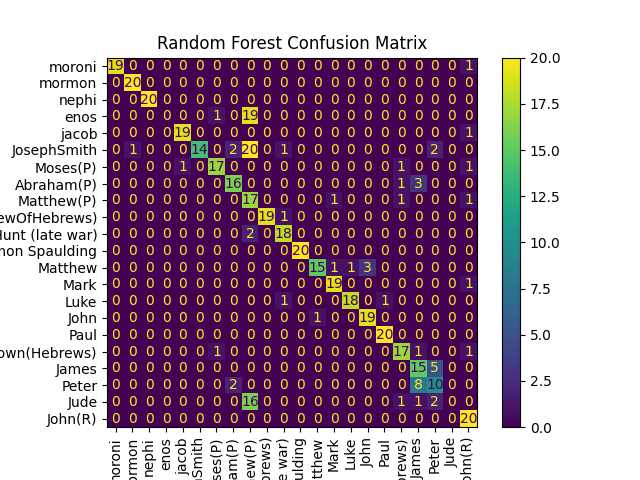
\includegraphics{Graphs/all/rf.png}

}

\caption{all Random Forest Confusion Matrix}

\end{figure}

\begin{itemize}
\tightlist
\item
  Accuracy: 0.7674
\item
  Precision: 0.7813
\item
  Recall: 0.7674
\item
  F1-Score: 0.7505
\end{itemize}

The numeric results aren't as strong, but when accounting for some
authors that have very little writings the results make more sense.

\hypertarget{word-comparisons}{%
\subsection{\texorpdfstring{\textbf{Word
Comparisons}}{Word Comparisons}}\label{word-comparisons}}

Another way to analyze authorship would be to visualize function word
use percentages in a scatterplot. I plot two words at a time as some
words have a correlation in usage. Some have no correlation and are
simply just a means to showcase more data at once. An important factor
to look at is groupings. I divided authorship by color. The Book of
Mormon authors are shades of blue, Joseph Smith is black and The Late
War, The Spaulding Manuscript and The Late War are red. Some words show
tighter groupings between those different authorships and some show no
much correlation. Below are a diverse amount of word combinations
showing the different correlations:

\begin{figure}

{\centering 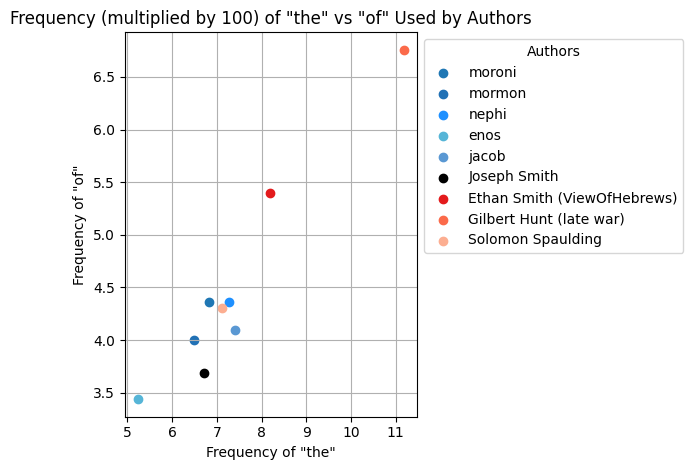
\includegraphics{Graphs/Word Comparisons/the_of_output.png}

}

\caption{the of combination}

\end{figure}

\begin{figure}

{\centering 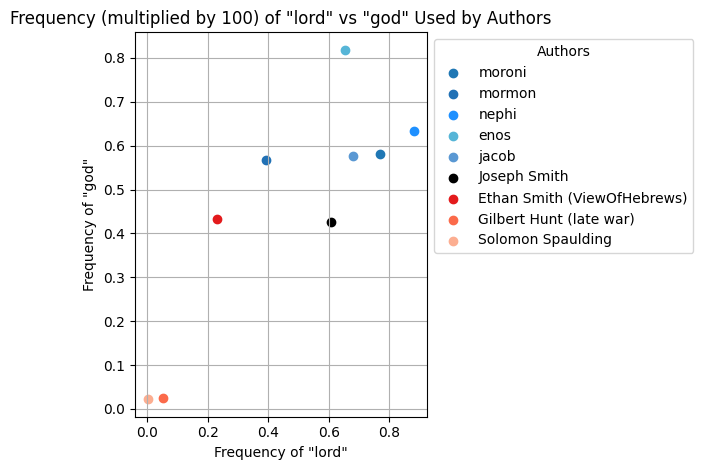
\includegraphics{Graphs/Word Comparisons/lord_god_output.png}

}

\caption{lord god combination}

\end{figure}

\begin{figure}

{\centering 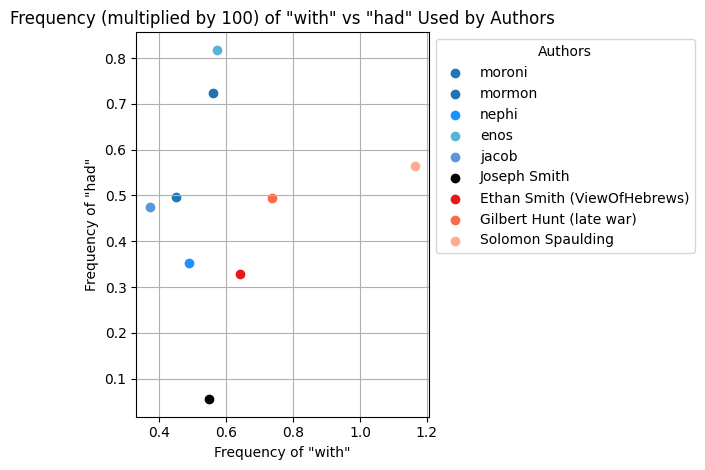
\includegraphics{Graphs/Word Comparisons/with_had_output.png}

}

\caption{with had combination}

\end{figure}

\begin{figure}

{\centering 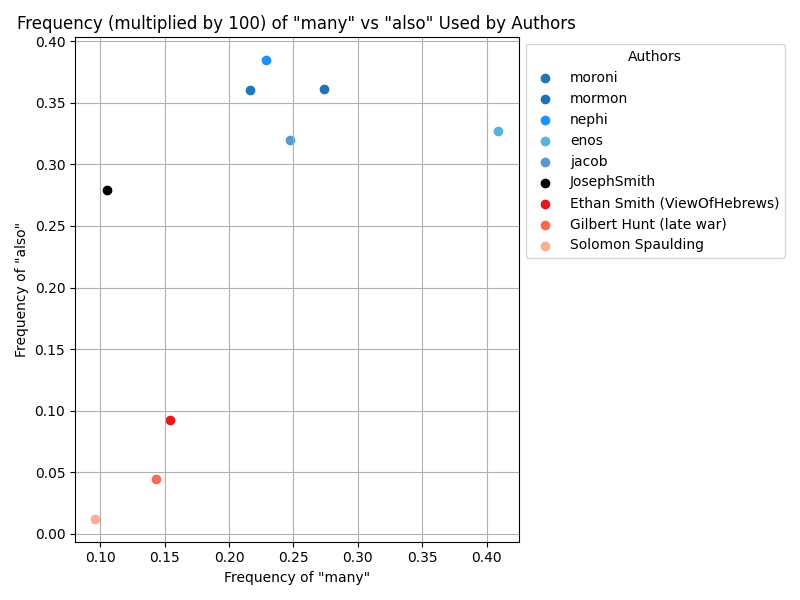
\includegraphics{Graphs/Word Comparisons/many_also_output.png}

}

\caption{many also combination}

\end{figure}

\begin{figure}

{\centering 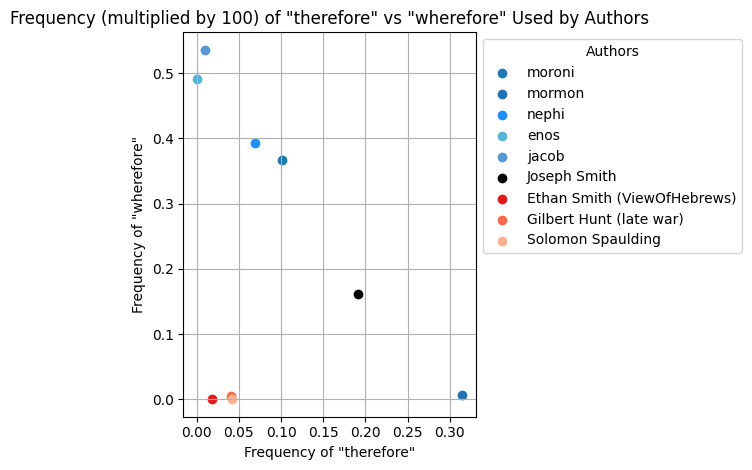
\includegraphics{Graphs/Word Comparisons/therefore_wherefore_output.png}

}

\caption{therefore wherefore combination}

\end{figure}

\begin{figure}

{\centering 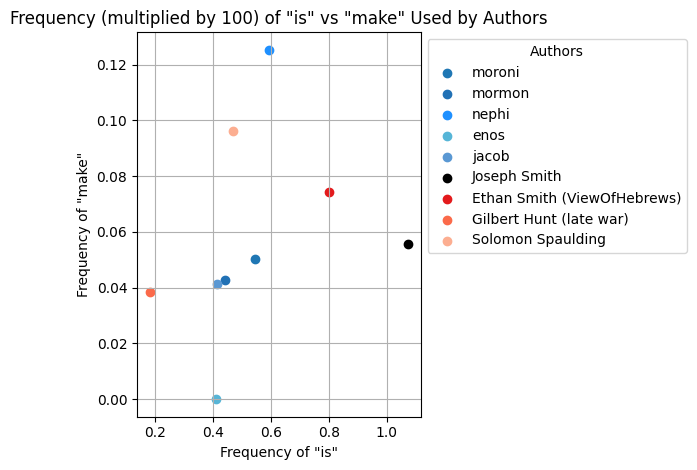
\includegraphics{Graphs/Word Comparisons/is_make_output.png}

}

\caption{is make combination}

\end{figure}

\begin{figure}

{\centering 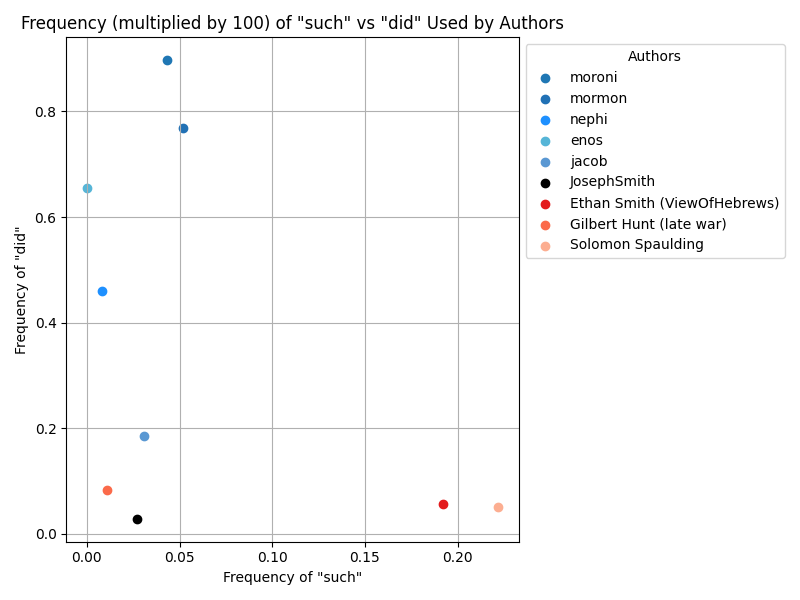
\includegraphics{Graphs/Word Comparisons/such_did_output.png}

}

\caption{such did combination}

\end{figure}

\begin{figure}

{\centering 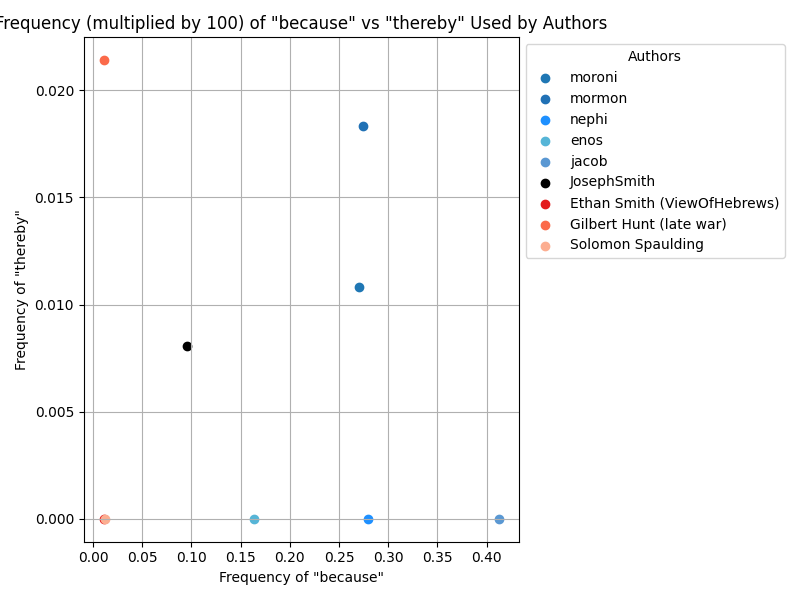
\includegraphics{Graphs/Word Comparisons/because_thereby_output.png}

}

\caption{because thereby combination}

\end{figure}

\begin{figure}

{\centering 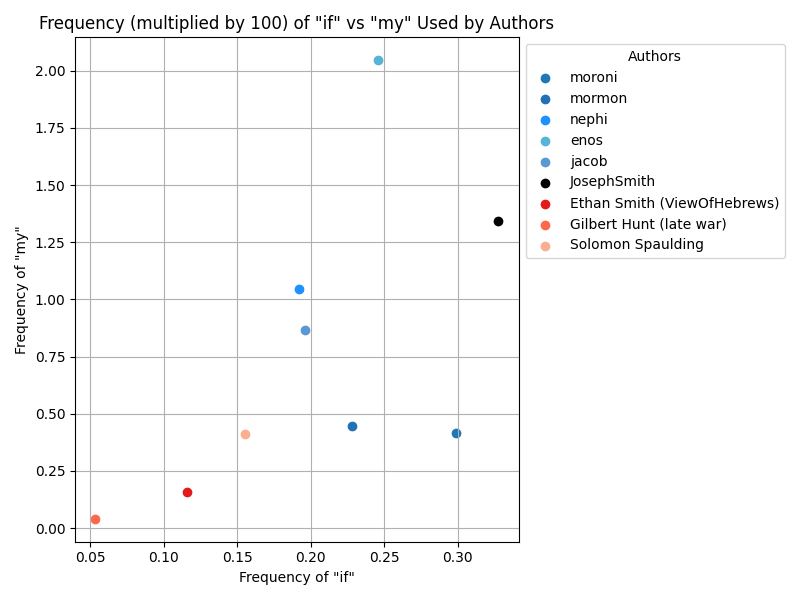
\includegraphics{Graphs/Word Comparisons/if_my_output.png}

}

\caption{if my combination}

\end{figure}

\begin{figure}

{\centering 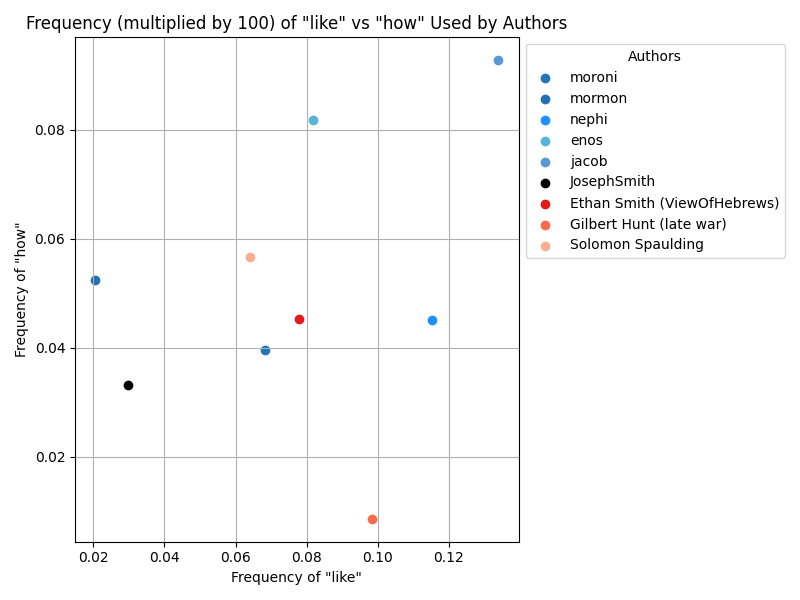
\includegraphics{Graphs/Word Comparisons/like_how_output.png}

}

\caption{like how combination}

\end{figure}

\begin{figure}

{\centering 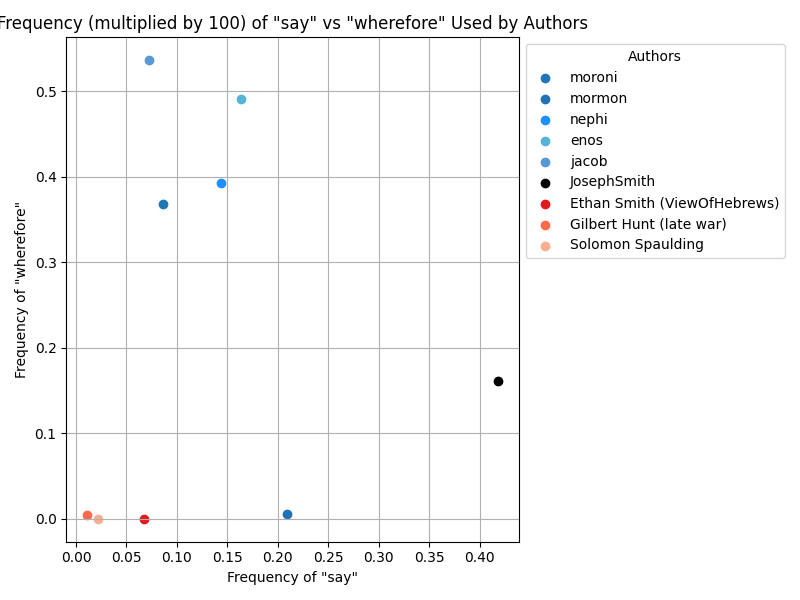
\includegraphics{Graphs/Word Comparisons/say_wherefore_output.png}

}

\caption{say wherefore combination}

\end{figure}

Graphs based off of other stylometric variables (average letter per
word, average words per sentence, vowel usage) also provide some
interesting insights

\begin{figure}

{\centering 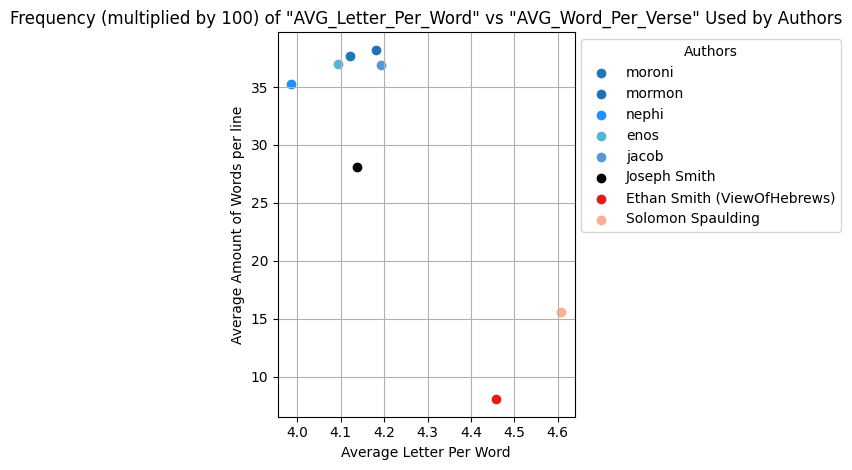
\includegraphics{Graphs/Word Comparisons/avg_output.png}

}

\caption{avg}

\end{figure}

\begin{figure}

{\centering 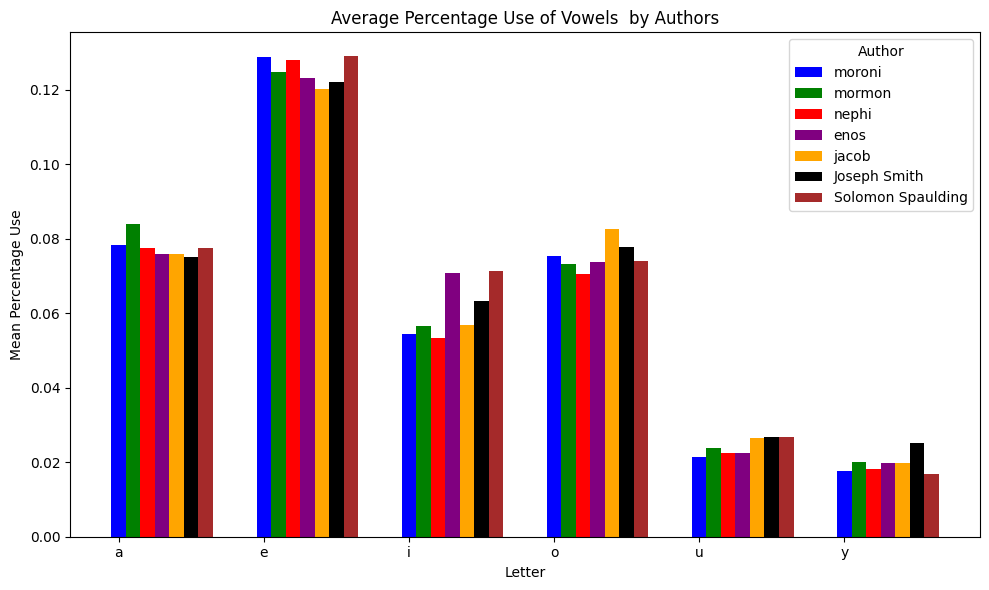
\includegraphics{Graphs/Word Comparisons/vowel_output.png}

}

\caption{vowels}

\end{figure}

In a good amount of the graphs there seems to be a grouping between The
Book of Mormon authors and the other authors. This does seem to lend
support towards the idea that The Book of Mormon has a somewhat
consistent usage of function words throughout the whole text. Critics of
The Book of Mormon could say this is evidence of Joseph Smith being the
sole author of The Book of Mormon. Authors of The Book of Mormon do
claim that due to the nature of the writing process, as in writing on
metal plates, they had to write in a language that they viewed as
limited and thus also limits their writing. Whether or not this
contributes to the similarities in function word use between The Book of
Mormon authorship cannot be concluded, but it is an explanation that
someone who holds to the religious view of The Book of Mormon could
take.

\hypertarget{conclusion}{%
\subsection{Conclusion}\label{conclusion}}

In exploration of authorship of The Book of Mormon and different text we
find evidence through stylometric analysis that the claims Joseph Smith
and The Book of Mormon itself claim about the authorship of The Book of
Mormon may have truth to them. When using machine learning models to
learn the patterns of the different authors and then make predictions
based off those patterns, a machine learning model can predict accuracy
up to high percentage. When looking at function word usage individually
we can see that there is some grouping in The Book of Mormon authors in
how they use function words, but unique patterns still do present
themselves among certain vocabulary. The miraculous claims of authorship
regarding The Book of Mormon is not something that can be proven, but by
investigating the claims made we can find evidence that does lend to
multiple authors of The Book of Mormon.

\hypertarget{references}{%
\subsubsection{References}\label{references}}

\begin{itemize}
\tightlist
\item
  \href{https://languages.oup.com/google-dictionary-en}{Oxford
  Languages}
\item
  \href{https://guides.temple.edu/stylometryfordh/methods}{Stylometry
  Techniques}
\item
  \href{https://www.churchofjesuschrist.org/study/scriptures/bofm?lang=eng}{The
  Book Of Mormon Text}
\item
  \href{https://aclanthology.org/W14-0908.pdf}{Function Word Usage In
  Determining Authorship Article}
\end{itemize}

\begin{center}\rule{0.5\linewidth}{0.5pt}\end{center}

\hypertarget{appendicesv}{%
\subsubsection{Appendicesv}\label{appendicesv}}

\begin{itemize}
\tightlist
\item
  \textbf{Appendix A}:
  \href{Data_organizing_transformation.ipynb}{Jupyter Notebook File Of
  Data Preprocessing}
\item
  \textbf{Appendix B}: \href{ML_Model_Usage.ipynb}{Jupyter Notebook File
  Of Machine Learning Process}
\item
  \textbf{Appendix C}: \href{Data_visualizations.ipynb}{Jupyter Notebook
  File Of Visualizations Creation (Some also found in Appendix B)}
\item
  \textbf{Appendix D}: \href{Graphs}{All Visualizations}
\item
  \textbf{Appendix E}: \href{texts}{All Text}
\item
  \textbf{Appendix F}: \href{~$metrics_report.xlsx}{All Numeric Metrics}
\end{itemize}



\end{document}
